\documentclass[]{article}
\usepackage{lmodern}
\usepackage{amssymb,amsmath}
\usepackage{ifxetex,ifluatex}
\usepackage{fixltx2e} % provides \textsubscript
\ifnum 0\ifxetex 1\fi\ifluatex 1\fi=0 % if pdftex
  \usepackage[T1]{fontenc}
  \usepackage[utf8]{inputenc}
\else % if luatex or xelatex
  \ifxetex
    \usepackage{mathspec}
  \else
    \usepackage{fontspec}
  \fi
  \defaultfontfeatures{Ligatures=TeX,Scale=MatchLowercase}
\fi
% use upquote if available, for straight quotes in verbatim environments
\IfFileExists{upquote.sty}{\usepackage{upquote}}{}
% use microtype if available
\IfFileExists{microtype.sty}{%
\usepackage{microtype}
\UseMicrotypeSet[protrusion]{basicmath} % disable protrusion for tt fonts
}{}
\usepackage[margin=1in]{geometry}
\usepackage{hyperref}
\hypersetup{unicode=true,
            pdftitle={Comparative mortality trends, indexed to 1981, by broad age groups},
            pdfauthor={Jon Minton},
            pdfborder={0 0 0},
            breaklinks=true}
\urlstyle{same}  % don't use monospace font for urls
\usepackage{longtable,booktabs}
\usepackage{graphicx,grffile}
\makeatletter
\def\maxwidth{\ifdim\Gin@nat@width>\linewidth\linewidth\else\Gin@nat@width\fi}
\def\maxheight{\ifdim\Gin@nat@height>\textheight\textheight\else\Gin@nat@height\fi}
\makeatother
% Scale images if necessary, so that they will not overflow the page
% margins by default, and it is still possible to overwrite the defaults
% using explicit options in \includegraphics[width, height, ...]{}
\setkeys{Gin}{width=\maxwidth,height=\maxheight,keepaspectratio}
\IfFileExists{parskip.sty}{%
\usepackage{parskip}
}{% else
\setlength{\parindent}{0pt}
\setlength{\parskip}{6pt plus 2pt minus 1pt}
}
\setlength{\emergencystretch}{3em}  % prevent overfull lines
\providecommand{\tightlist}{%
  \setlength{\itemsep}{0pt}\setlength{\parskip}{0pt}}
\setcounter{secnumdepth}{0}
% Redefines (sub)paragraphs to behave more like sections
\ifx\paragraph\undefined\else
\let\oldparagraph\paragraph
\renewcommand{\paragraph}[1]{\oldparagraph{#1}\mbox{}}
\fi
\ifx\subparagraph\undefined\else
\let\oldsubparagraph\subparagraph
\renewcommand{\subparagraph}[1]{\oldsubparagraph{#1}\mbox{}}
\fi

%%% Use protect on footnotes to avoid problems with footnotes in titles
\let\rmarkdownfootnote\footnote%
\def\footnote{\protect\rmarkdownfootnote}

%%% Change title format to be more compact
\usepackage{titling}

% Create subtitle command for use in maketitle
\newcommand{\subtitle}[1]{
  \posttitle{
    \begin{center}\large#1\end{center}
    }
}

\setlength{\droptitle}{-2em}

  \title{Comparative mortality trends, indexed to 1981, by broad age groups}
    \pretitle{\vspace{\droptitle}\centering\huge}
  \posttitle{\par}
    \author{Jon Minton}
    \preauthor{\centering\large\emph}
  \postauthor{\par}
    \date{}
    \predate{}\postdate{}
  
\usepackage{booktabs}
\usepackage{longtable}
\usepackage{array}
\usepackage{multirow}
\usepackage[table]{xcolor}
\usepackage{wrapfig}
\usepackage{float}
\usepackage{colortbl}
\usepackage{pdflscape}
\usepackage{tabu}
\usepackage{threeparttable}
\usepackage{threeparttablex}
\usepackage[normalem]{ulem}
\usepackage{makecell}

\begin{document}
\maketitle

\section{Introduction}\label{introduction}

This short report shows how mortality rates have changed in Scotland,
for males and females separately, for a number of broadly defined age
groups. Mortality rates are shown indexed to their value in 1981.
(e.g.~a value of 70 means the mortality rate for that particular age
group was 70\% of their rate in 1981, and so on.) Mortality rate indixes
are also presented for three other countries/country groups (HMD codes
shown in parentheses):

\begin{itemize}
\tightlist
\item
  England \& Wales (GBRTENW)
\item
  France (FRANTP)
\item
  United States (USA)
\end{itemize}

\section{Methodology}\label{methodology}

All data were extracted from the Human Mortality Database (HMD). The
mortality rates at each age in single years were calculated from the
population exposures and numbers of deaths. A small continuity
correction of 5 was added to the numerators and denominators before
calculating age-specific mortality rates.

Each age-specific mortality rate was then indexed to its value in 1981
so that, for example, a value of 110 means a death rate 10\% higher than
that in 1981, and a value of 90 means a death rate 90\% of that observed
in 1981. These age-specific mortality indices were then weighted to
produce indices for a smaller number of broader age categories using the
following approach:

\begin{itemize}
\tightlist
\item
  Each age in single years was assigned to a broader age category
  comprising multiple ages in single years;
\item
  The proportion of the population at each age in single years within
  each specific broad age category, in each specific year, was
  calculated to produce a within-category weighting factor;
\item
  For each year, and each age category, the age-specific mortality
  indices were multiplied by the weighted factors, then summed, in order
  to produce a year-specific population weighted mortality index for
  that age group.
\end{itemize}

The age categories are as follows:

\begin{itemize}
\tightlist
\item
  0 to 14 years
\item
  15 to 34 years
\item
  35 to 54 years
\item
  55 to 74 years
\item
  75 to 89 years
\item
  90 years and above (up to 110 years of age exclusive)
\end{itemize}

This approach was used in order to adjust for changes in within-age
category population structure, which could lead to mortality rates
changing for artefactual reasons alone. For example, if the average age
within the 55 to 74 year old age strata changes from (say) 62 to 65
between 1981 and 1991, then the overall crude mortality rate within this
strata could increase through change in population composition alone,
even if the mortality rates at each age in single years within this
strata have fallen.

The above calculations were produced separately for each of the
countries, and within each country for males and females separately.

\begin{verbatim}
## Parsed with column specification:
## cols(
##   code = col_character(),
##   Year = col_integer(),
##   Age = col_integer(),
##   gender = col_character(),
##   num_deaths = col_double(),
##   num_population = col_double(),
##   exposure = col_double()
## )
\end{verbatim}

\section{Results}\label{results}

Figures showing how the weighted indices changed since 1981 are shown
separately for females and males below.

\subsection{Figure for females}\label{figure-for-females}

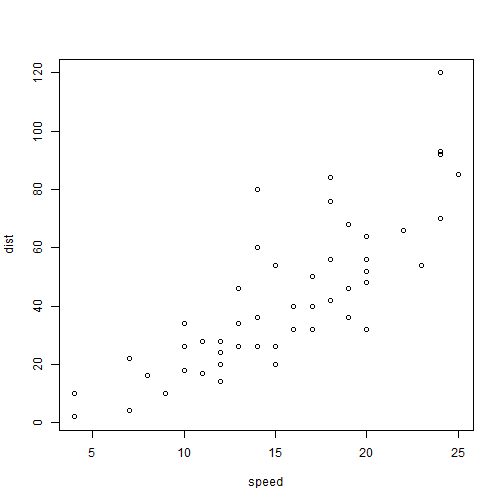
\includegraphics{indexed_trends_writeup_files/figure-latex/unnamed-chunk-3-1.pdf}

\subsection{Figure for males}\label{figure-for-males}

\includegraphics{indexed_trends_writeup_files/figure-latex/unnamed-chunk-4-1.pdf}

\subsection{Discussion of results}\label{discussion-of-results}

There has been a clear trend towards towards falling mortality rates in
all countries, and for both males and females, but there are also clear
differences by age group, gender and country. This discussion will look
at each age group, from infants and children at the start of the life
course, to the very elderly at the end of the life course, and within
each age category discuss the general trends, gender differences, and
how Scotland compares with the other countries selected.

\subsubsection{Infants and young
children}\label{infants-and-young-children}

Weighted mortality rate indices have fallen faster amongst 0-14 year
olds than amongst any other age groups, for males and females, in every
country \emph{except Scotland} since 1981. The following table shows how
the weighted index has changed since 1981 for each population under
consideration.

\begin{longtable}[]{@{}llrrrr@{}}
\caption{Weighted index of mortality rates in 0-14 year olds (1981 =
100), selected countries.}\tabularnewline
\toprule
country & gender & 1990 & 2000 & 2010 & 2016\tabularnewline
\midrule
\endfirsthead
\toprule
country & gender & 1990 & 2000 & 2010 & 2016\tabularnewline
\midrule
\endhead
Scotland & Female & 92 & 75 & 70 & 73\tabularnewline
Scotland & Male & 94 & 72 & 62 & 63\tabularnewline
England \& Wales & Female & 78 & 54 & 47 & 39\tabularnewline
England \& Wales & Male & 79 & 53 & 40 & 33\tabularnewline
France & Female & 68 & 50 & 35 & 32\tabularnewline
France & Male & 66 & 47 & 31 & 28\tabularnewline
United States & Female & 83 & 64 & 48 & 50\tabularnewline
United States & Male & 79 & 57 & 42 & 42\tabularnewline
\bottomrule
\end{longtable}

Within this age group, mortality rates fell to to between 60-70\% of
their 1981 rates in Scotland, compared to around 30-40\% in France, and
40-50\% in England \& Wales and the USA.

Though the trends in mortality rate improvements in these age groups
have been less favourable in Scotland than in these other populations,
only a small proportion of all deaths that occur, occur in infancy and
childhood, so these trends alone do little to explain either Scotland's
relative disadvantage in longevity overall, or differences in trends
after around 2012.

\subsubsection{Older children and younger adults (15-34 year
olds)}\label{older-children-and-younger-adults-15-34-year-olds}

The trends in this age group are generally less favourable than other
age groups in each of the populations being compared, and are
particularly unfavourable in Scotland. Whereas the trends in most other
age groups have been towards considerable improvements ( falling
mortality rates) since 1981, in this age group there is more evidence of
stalling in the other countries, and worsening in Scotland. The table
below shows how index values in this age group compares in the eight
population groups of interest.

\begin{table}

\caption{\label{tab:unnamed-chunk-6}Weighted index of mortality rates in 15-34 year olds (1981 = 100), selected countries.}
\centering
\begin{tabular}[t]{l|l|r|r|r|r}
\hline
country & gender & 1990 & 2000 & 2010 & 2016\\
\hline
Scotland & Female & 95 & 107 & 105 & 97\\
\hline
Scotland & Male & 102 & 112 & 93 & 84\\
\hline
England \& Wales & Female & 89 & 84 & 68 & 67\\
\hline
England \& Wales & Male & 106 & 96 & 71 & 68\\
\hline
France & Female & 83 & 64 & 45 & 42\\
\hline
France & Male & 96 & 68 & 50 & 40\\
\hline
United States & Female & 95 & 82 & 75 & 89\\
\hline
United States & Male & 101 & 73 & 67 & 80\\
\hline
\end{tabular}
\end{table}

Mortality rates in these age groups were between a tenth and an eighth
higher in Scotland by 2000 compared with 1981, and by 2016 fell only
marginally for women, and to around 85\% of their 1981 values in
Scotland. At their peak, in the late 1990s/early 2000s, mortality rates
in males were around a fifth higher, and in females a tenth higher, than
in 1981.

Trends had also stalled in the USA throughout the 1980s, before falling
in the early/mid 1990s. Mortality rates also remained stalled in England
\& Wales for males, before improving in the mid/late 1990s, and
continued to improve for females; by 2016 mortality rate improvements
had become roughly equal for both gender. In France, the mid 1990s
marked an acceleration in improvements for both genders, which continued
in subsequent periods, such that by 2016 mortality rates in this age
group were less than half their level in 1981.

\subsubsection{Middle working age (35-54 year
olds)}\label{middle-working-age-35-54-year-olds}

Mortality rate improvements in the middle of working age have tended to
be more persistent in this age group than in the 15-34 year old age
group, with more gradual improvements observed in each country and both
genders. \emph{However, it is also within this age group that sudden
changes towards either stagnation (England/Wales) or worsenings
(Scotland, and to a lesser extent USA) since around 2012 can be
observed.} The increase in mortality rates between 2010 and 2016 can be
seen in the graphs above, and the table below.

\begin{table}

\caption{\label{tab:unnamed-chunk-7}Weighted index of mortality rates in 35-54 year olds (1981 = 100), selected countries.}
\centering
\begin{tabular}[t]{l|l|r|r|r|r}
\hline
country & gender & 1990 & 2000 & 2010 & 2016\\
\hline
Scotland & Female & 90 & 80 & 71 & 78\\
\hline
Scotland & Male & 80 & 76 & 68 & 74\\
\hline
England \& Wales & Female & 84 & 76 & 65 & 62\\
\hline
England \& Wales & Male & 88 & 79 & 70 & 66\\
\hline
France & Female & 84 & 78 & 65 & 55\\
\hline
France & Male & 92 & 76 & 58 & 48\\
\hline
United States & Female & 89 & 86 & 80 & 85\\
\hline
United States & Male & 98 & 81 & 70 & 75\\
\hline
\end{tabular}
\end{table}

In Scotland, mortality rates in this age group increased by almost a
tenth in both males and females between 2010 and 2016. In the USA, they
increased by around an eighth. Over the same period, they fell by around
5\% in England \& Wales, and around 15-20\% in France.

\subsubsection{Late working age and early retirement ages (55-74 years
of
age)}\label{late-working-age-and-early-retirement-ages-55-74-years-of-age}

Mortality rates in this age group have seen the fastest rates of
improvement in Scotland since 1981, compared with other popualtion
groups, but have been stalling in recent years. They fell by around
10-15\% from 1981 to 1990, by around 20\% from 1990 to 2000, by around a
quarter from 2000 to 2010, but by only around 8-10\% between 2010 and
2016. Though this latter comparison is of a shorter time period, a
slowdown in the trends seems evident from the figures.

Similar slowdowns are also seen in England \& Wales, and France, and
flattening mortality improvements have been observed in the USA.

\begin{table}

\caption{\label{tab:unnamed-chunk-8}Weighted index of mortality rates in 55-74 year olds (1981 = 100), selected countries.}
\centering
\begin{tabular}[t]{l|l|r|r|r|r}
\hline
country & gender & 1990 & 2000 & 2010 & 2016\\
\hline
Scotland & Female & 90 & 71 & 57 & 53\\
\hline
Scotland & Male & 84 & 68 & 49 & 44\\
\hline
England \& Wales & Female & 89 & 70 & 55 & 53\\
\hline
England \& Wales & Male & 82 & 60 & 45 & 41\\
\hline
France & Female & 79 & 67 & 60 & 58\\
\hline
France & Male & 83 & 67 & 56 & 51\\
\hline
United States & Female & 94 & 86 & 71 & 71\\
\hline
United States & Male & 86 & 71 & 59 & 60\\
\hline
\end{tabular}
\end{table}

\subsubsection{Central retirement ages (75-89 year
olds)}\label{central-retirement-ages-75-89-year-olds}

The table below shows the index values for this age group in each of the
population gruops.

\begin{table}

\caption{\label{tab:unnamed-chunk-9}Weighted index of mortality rates in 75-89 year olds (1981 = 100), selected countries.}
\centering
\begin{tabular}[t]{l|l|r|r|r|r}
\hline
country & gender & 1990 & 2000 & 2010 & 2016\\
\hline
Scotland & Female & 90 & 82 & 66 & 63\\
\hline
Scotland & Male & 89 & 73 & 56 & 51\\
\hline
England \& Wales & Female & 86 & 77 & 61 & 57\\
\hline
England \& Wales & Male & 87 & 72 & 52 & 49\\
\hline
France & Female & 76 & 62 & 49 & 44\\
\hline
France & Male & 80 & 68 & 53 & 47\\
\hline
United States & Female & 93 & 93 & 77 & 73\\
\hline
United States & Male & 92 & 83 & 65 & 61\\
\hline
\end{tabular}
\end{table}

Within this age band, the relative improvements between 1981 and 2016
were larger for males than females in Scotland (51 for males compared
with 63 for females), in England \& Wales (49 compared with 57), and in
the USA (61 comapred with 73), whereas in France the index of
improvement was slightly greater in females (44) than males.

There have been very consistent trends in mortality rate improvement in
both genders and all four countries in this age group. However, annual
rates of improvement have been more modest in recent years. The table
below shows the average change in the index values for each of the eight
population groups over the 1980s, 1990s, 2000s, and between 2010 and
2016. With the exception of females in the 1980s, average rates of
annual improvement have been substantially less in the 2010-2016 period
than in earlier decades. In Scotland, annual improvements in the 2000s
were around three times larger than improvements over this latter period
in women, and around twice as large in men. The equivalent relative
improvement ratios, were around 2.6 times (females) and 3.0 times
(males) in England \& Wales, 1.7 (females) and 1.4 (males) in France,
and around 2.5 times greater in the USA for both males and females.

\begin{table}

\caption{\label{tab:unnamed-chunk-10}Average annual change in index values for 75-89 year olds, by period, selected countries.}
\centering
\begin{tabular}[t]{l|l|r|r|r|r}
\hline
country & gender & 1980s & 1990s & 2000s & 2010-2016\\
\hline
Scotland & Female & -1.11 & -0.83 & -1.56 & -0.53\\
\hline
Scotland & Male & -1.26 & -1.53 & -1.72 & -0.84\\
\hline
England \& Wales & Female & -1.55 & -0.93 & -1.64 & -0.63\\
\hline
England \& Wales & Male & -1.53 & -1.50 & -1.93 & -0.64\\
\hline
France & Female & -2.33 & -1.42 & -1.30 & -0.75\\
\hline
France & Male & -1.98 & -1.21 & -1.45 & -1.07\\
\hline
United States & Female & -1.05 & 0.02 & -1.60 & -0.63\\
\hline
United States & Male & -1.07 & -0.90 & -1.75 & -0.70\\
\hline
\end{tabular}
\end{table}

Though there have not been clear increases in mortality risks in this
age group, because a large proportion of all deaths that occur, tend to
occur in these age groups, the clear slowdown in improvements in this
age group is likely to be an important driver of falling and stalling
life expectancies. The international comparison shows that, unlike the
trends in some younger age groups, this phenomenon is not specific to
Scotland.

\subsubsection{Older pensioners (90 year olds and
above)}\label{older-pensioners-90-year-olds-and-above}

The table below shows the index values for this age group in each of the
population groups. General tendencies towards continually improving
mortality at these ages were observed for Scotland, England \& Wales,
and France since the early 1980s, but not in the USA, where mortality
rates increased modestly until the early 2000s, before starting to fall.
In Scotland, England \& Wales, and France there are indications of
stalling improvements after around 2010-2012, consistent with that
observed in the previous age groups, whereas trends in the USA are
continuing to improve as they catch up towards the other three
countries.

\begin{table}

\caption{\label{tab:unnamed-chunk-11}Weighted index of mortality rates in 90 year olds and above (1981 = 100), selected countries.}
\centering
\begin{tabular}[t]{l|l|r|r|r|r}
\hline
country & gender & 1990 & 2000 & 2010 & 2016\\
\hline
Scotland & Female & 93 & 87 & 83 & 81\\
\hline
Scotland & Male & 91 & 82 & 80 & 74\\
\hline
England \& Wales & Female & 90 & 87 & 79 & 77\\
\hline
England \& Wales & Male & 92 & 88 & 76 & 72\\
\hline
France & Female & 87 & 77 & 67 & 65\\
\hline
France & Male & 91 & 84 & 73 & 69\\
\hline
United States & Female & 96 & 106 & 94 & 85\\
\hline
United States & Male & 100 & 106 & 93 & 80\\
\hline
\end{tabular}
\end{table}

The table below shows the average annual change in index values over the
1980s, 1990s, 2000s, and the period 2010-2016. This illustrates some
additional complications in the trends. As with males and females in the
USA, there is some evidence of `catch up' in the latest period for males
in Scotland, with a \emph{higher} average rate of improvement for males
in the 2010s than the 2000s; for Scottish females, the rates of
improvement are similar in the 2010s than the 2000s.

In France, and in England \& Wales, average rates of improvement in the
2010s were considerably smaller than in the 2000s, whereas improvements
accelerated over the latter compared with previous period for both
genders in the USA.

\begin{table}

\caption{\label{tab:unnamed-chunk-12}Average annual change in index values for 90 year olds and older, by period, selected countries.}
\centering
\begin{tabular}[t]{l|l|r|r|r|r}
\hline
country & gender & 1980s & 1990s & 2000s & 2010-2016\\
\hline
Scotland & Female & -0.78 & -0.52 & -0.40 & -0.44\\
\hline
Scotland & Male & -0.98 & -0.95 & -0.13 & -1.12\\
\hline
England \& Wales & Female & -1.09 & -0.32 & -0.80 & -0.29\\
\hline
England \& Wales & Male & -0.80 & -0.40 & -1.17 & -0.68\\
\hline
France & Female & -1.23 & -0.98 & -0.99 & -0.37\\
\hline
France & Male & -0.78 & -0.66 & -1.09 & -0.71\\
\hline
United States & Female & -0.72 & 0.92 & -1.19 & -1.49\\
\hline
United States & Male & -0.43 & 0.64 & -1.31 & -2.19\\
\hline
\end{tabular}
\end{table}

\section{Summary}\label{summary}

This document has shown how the population weighted indices of mortality
change since 1981 differ between age groups and genders within Scotland
and three comparator populations. Overall, there have been marked
improvements in mortality in each of these age groups, but with
considerable variation between populations. Mortality trends in Scotland
departed most from the comparator countries in 15-34 year olds, and
improvements in infant and childhood mortality (0-14 years old), in
particular, have been much slower than in other countries. There is also
evidence of catch-up in mortality trends, however, such as within the
55-74 year old age strata.

In rich countries, majority of deaths occur at older ages, and so more
modest changes in trends at these older ages are likely to impact life
expectancy much more than larger changes at younger ages. Scotland has
been similar to the comparator countries in seeing slow downs in
mortality rate improvements in these older ages in the 2010s, though
there is also evidence of mortality rates increasing, rather than simply
falling more slowly, at many ages in Scotland in recent years.


\end{document}
